%-------------------------------------------------------------------------------
%                            BAB III
%               		METODOLOGI PENELITIAN
%-------------------------------------------------------------------------------
% \fancyhf{} 
% \fancyfoot[R]{\thepage}
\chapter{METODE PENENILITIAN}
%\thispagestyle{plain} % Halaman pertama bab menggunakan gaya plain
\section{Waktu dan Lokasi Penelitian}
Penelitian ini akan bertempat pada beberapa ruangan yang digunakan oleh mahasiswa Jurusan Informatika USK yang umumnya terletak pada lantai 3 blok A dan blok E Gedung Fakultas MIPA USK. Waktu yang dibutuhkan agar penelitian ini dapat di implementasikan adalah 4 bulan terhitung dari bulan Januari 2024 hingga Mei 2024.

\section{Alat dan Bahan}
Alat dan Bahan yang akan digunakan pada penelitian ini terdiri dari beberapa perangkat keras (\textit{hardware}) dan perangkat lunak (\textit{software}) yang dijabarkan sebagai berikut:

\begin{enumerate}
\item Perangkat Keras
	\begin{itemize}
	\item Laptop Lenovo Yoga C740 dengan RAM 16GB DDR4, Intel® Core™ i7-10710U. 1.10 - 4.70 GHz,\textit{Solid State State Drive} (SSD) 1TB.
	\end{itemize}

\item Perangkat Lunak
	\begin{itemize}
	\item Linux Debian Ubuntu 22.04 LTS
	\item Visual Studio Code 1.71.0
	\item Python 3.8.17
	\end{itemize}
\end{enumerate}
\newpage
\section{Metode Penelitian}
Metode penelitian yang dilakukan akan terdiri dari beberapa tahapan penelitian. Skema dari alur tahapan tersebut dapat dilihat pada Gambar \ref{alur_penelitian}.

\begin{figure}[H]
	\centering
	\frame{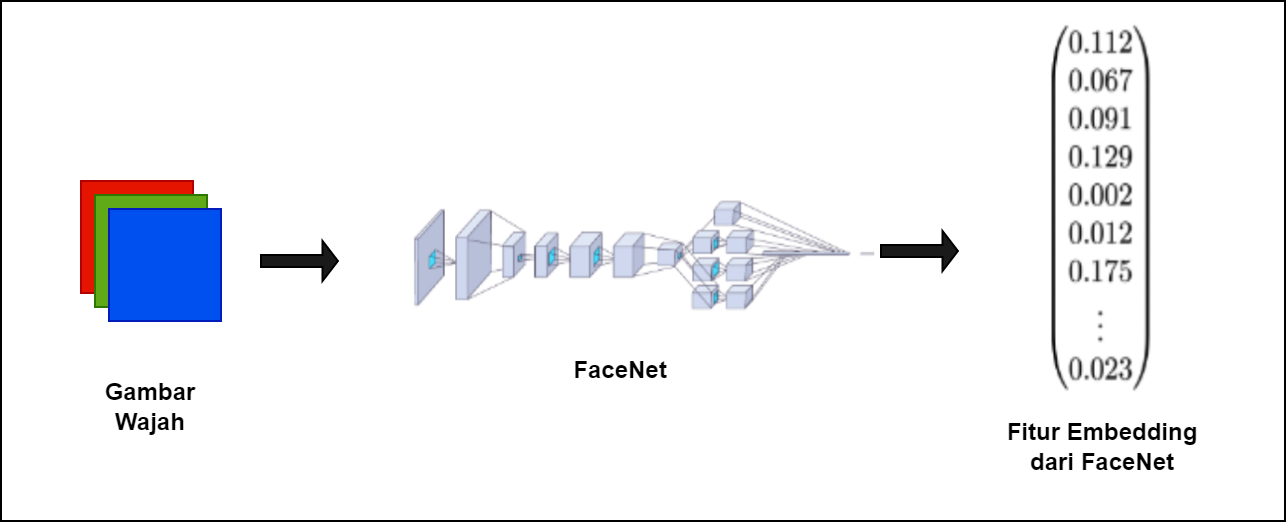
\includegraphics [width = 14cm, height= 5cm]{image/diagram_facenet}}
	\caption{\textit{Desain} Arsitektur \textit{FaceNet}}.
	\label{alur-penelitian} % cuman gambar dummy ya !
\end{figure}

%-----------------------------------------------------------------------------%

% Baris ini digunakan untuk membantu dalam melakukan sitasi
% Karena diapit dengan comment, maka baris ini akan diabaikan
% oleh compiler LaTeX.
\begin{comment}
\bibliography{daftar-pustaka}
\end{comment}